\subsection{Обзор существующих решений}

Анализ мобильных приложений проводится для того, чтобы выявить основные функциональные возможности, структуру и дизайн.
Для этого возьмем нескольких популярных мобильных приложений, включая
Wildberries \cite{AndroidWildberries},
OZ.by~\cite{AndroidOzBy},
LC Waikiki \cite{AndroidLcWaikiki},
Lamoda \cite{AndroidLamoda},
DeFacto \cite{AndroidDefacto}
и AliExpress \cite{AndroidAliExpress}.

Для анализа будут сделаны скриншоты главного экрана, экрана категорий, корзины, избранных, страницы с товаром, вид характеристик товара и входа в аккаунт
для каждого приложения.

Из анализа стало ясно, что у каждого приложения есть свои сильные и слабые стороны.
В целом, анализ мобильных приложений позволяет выявить недостатки и возможности для улучшения существующих приложений.

Главный экран в мобильном приложении по заказу товаров является первым взаимодействием пользователя с приложением.
Он должен быть удобным и информативным, чтобы привлечь внимание пользователя и помочь ему быстро найти нужный товар.
На главном экране обычно отображается список категорий товаров, актуальные предложения, новые поступления и лучшие продажи.
Также на главном экране может быть размещена поисковая строка, чтобы пользователь мог быстро найти интересующий его товар.
Важно, чтобы главный экран был интуитивно понятен и легко навигировался, чтобы пользователь мог быстро и легко перейти к нужному разделу приложения.

Аналоги главного экрана приведены на рисиснке~\ref{fig:analyzHome}.

Экран с номенклатурой в мобильном приложении - это страница, на которой пользователь может просмотреть полную информацию о товаре,
включая его название, описание, изображения, цену и характеристики.

Аналоги экрана с номенклатурой приведены на рисунке~\ref{fig:analyzItem}.

С другой стороны, экран с номенклатурой в мобильном приложении по заказу товаров - это страница,
на которой отображается список доступных для покупки товаров с их характеристиками,
ценами и возможностью добавления в корзину.
Покупателю нужно знать характеристики товаров,
чтобы сравнить и выбрать наиболее подходящий для своих нужд.
Это может включать в себя такие параметры, как размер, цвет, материал, вес и другие особенности товара.

Аналоги экрана с характеристиками приведены на рисунке~\ref{fig:analyzItemCharacteristic}.

\begin{figure}[!p]
  \centering

  \begin{minipage}{0.16\textwidth}
    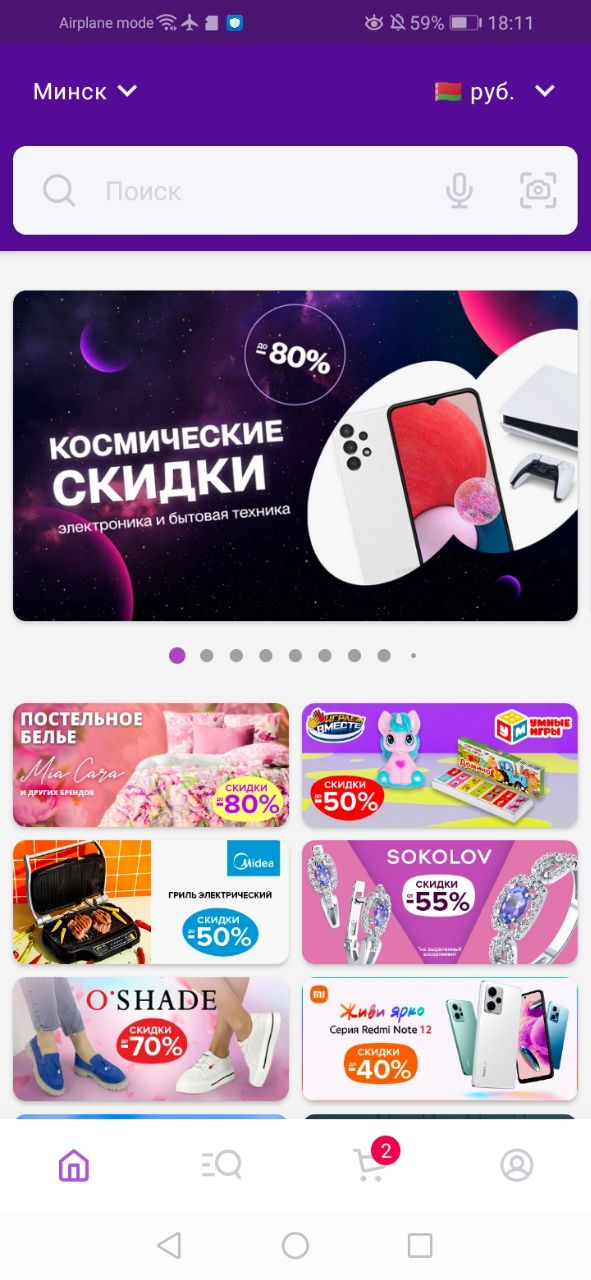
\includegraphics[width=.99\linewidth]
    {images/candidates/Wildberies/Home.jpg}
  \end{minipage}
  \begin{minipage}{0.16\textwidth}
    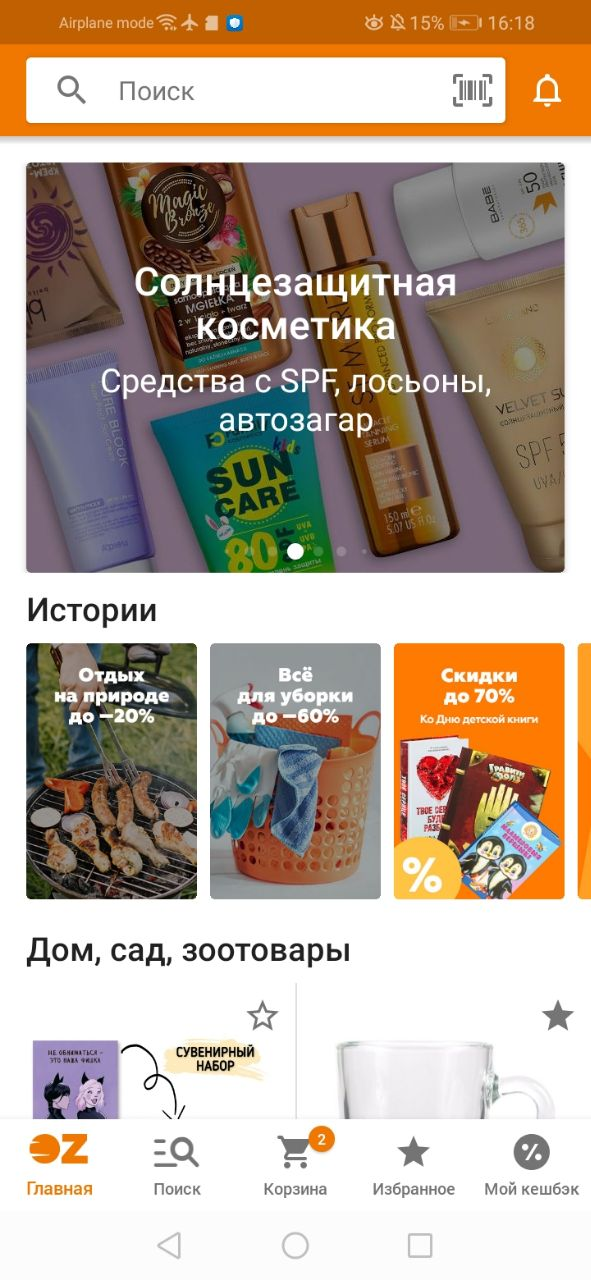
\includegraphics[width=.99\linewidth]
    {images/candidates/OZby/Home.jpg}
  \end{minipage}
  \begin{minipage}{0.16\textwidth}
    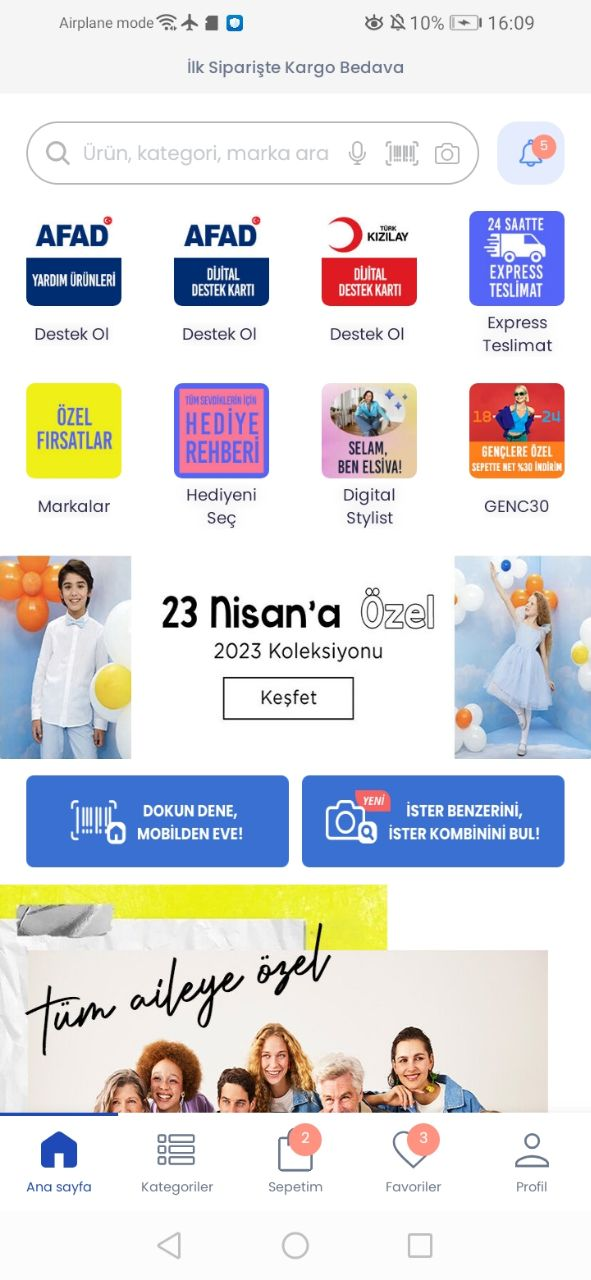
\includegraphics[width=.99\linewidth]
    {images/candidates/LCWaikiki/Home.jpg}
  \end{minipage}
  \begin{minipage}{0.16\textwidth}
    
\includegraphics[width=.99\linewidth]
    {images/candidates/Lamoda/Home.jpg}
  \end{minipage}
  \begin{minipage}{0.16\textwidth}
    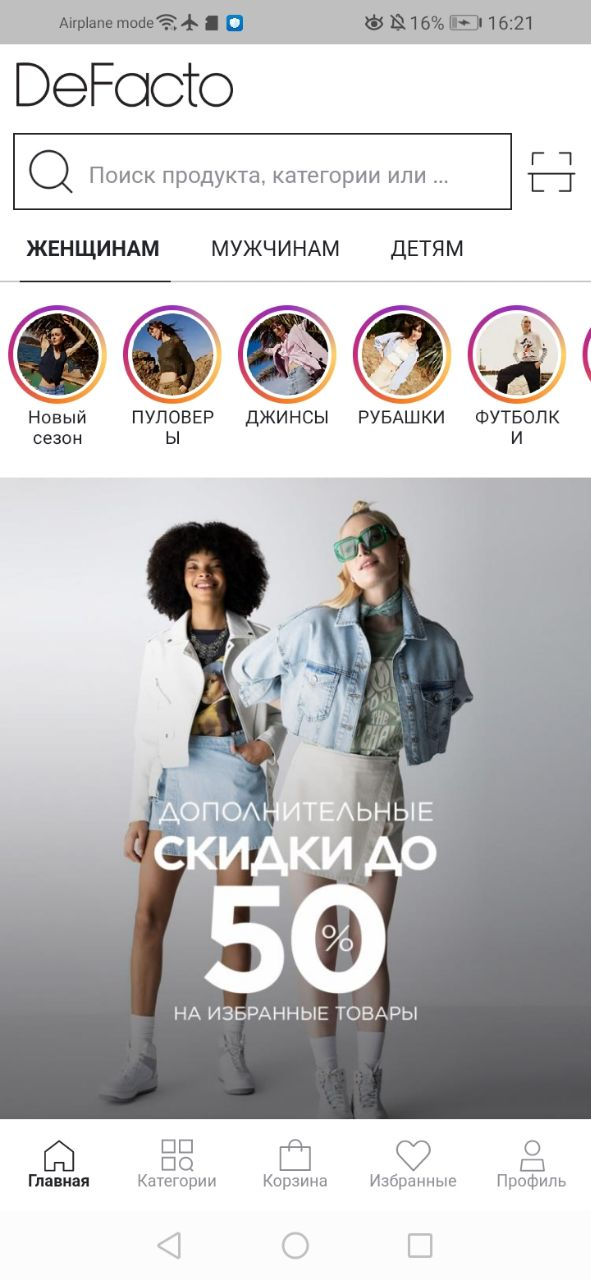
\includegraphics[width=.99\linewidth]
    {images/candidates/DeFacto/Home.jpg}
  \end{minipage}
  \begin{minipage}{0.16\textwidth}
    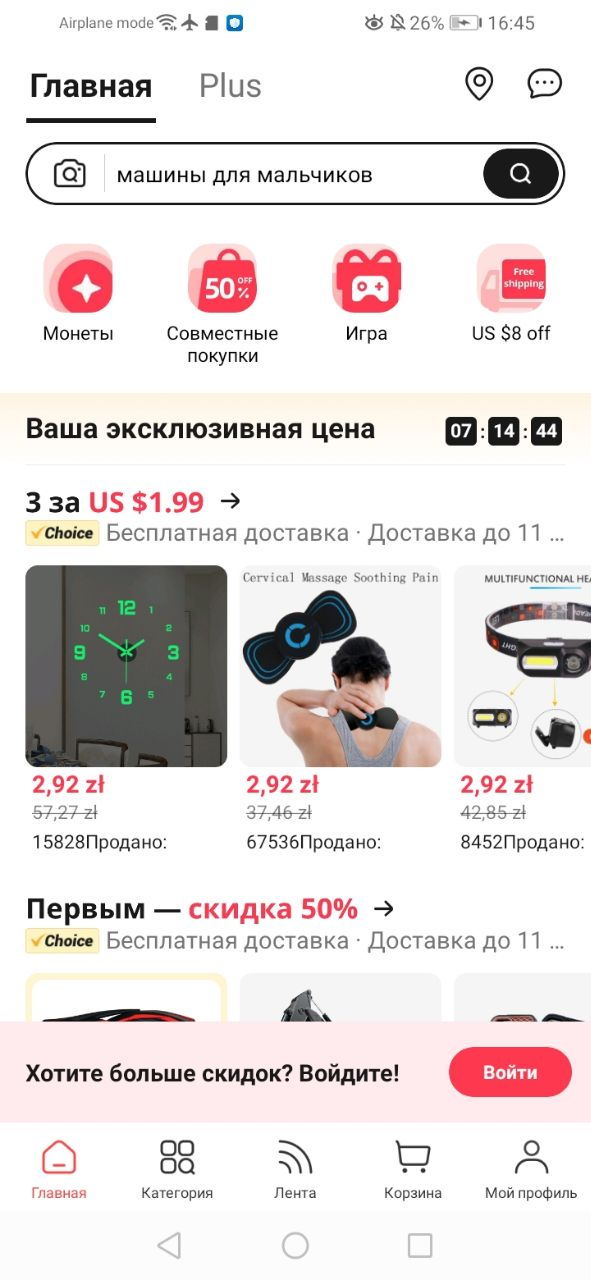
\includegraphics[width=.99\linewidth]
    {images/candidates/AliExpress/Home.jpg}
  \end{minipage}

  \caption{Аналоги главного экрана}\label{fig:analyzHome}
\end{figure}

\begin{figure}[!p]
  \centering

  \begin{minipage}{0.16\textwidth}
    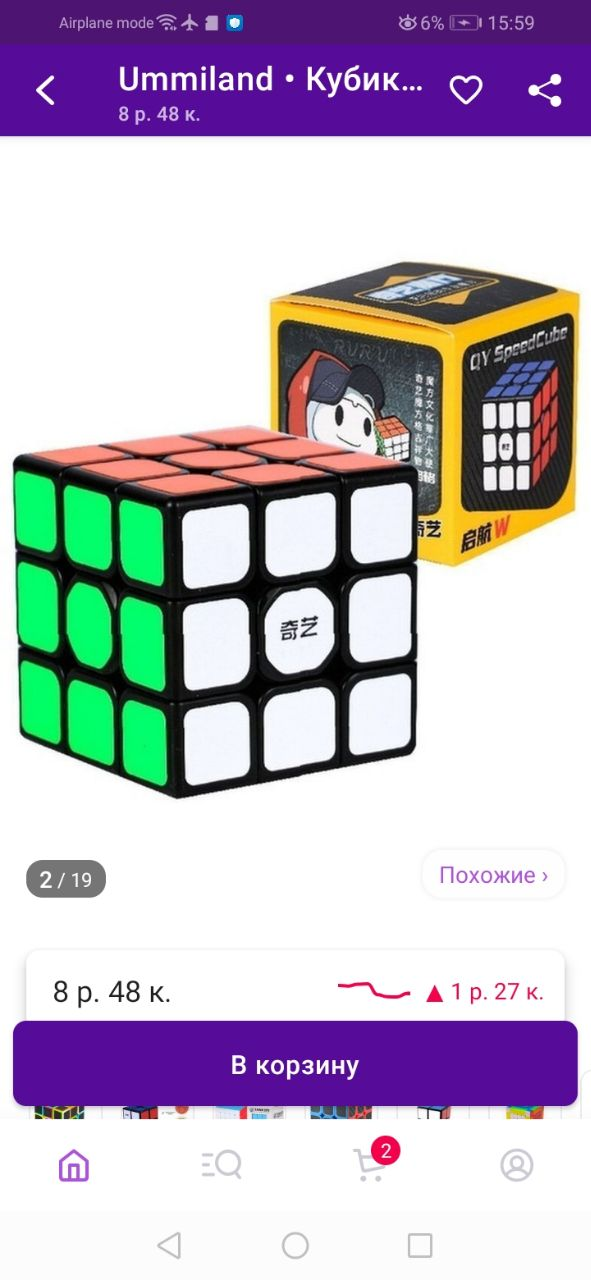
\includegraphics[width=.99\linewidth]
    {images/candidates/Wildberies/Item.jpg}
  \end{minipage}
  % \begin{minipage}{0.16\textwidth}
  %   \includegraphics[width=.99\linewidth]
  %   {images/candidates/OZby/Item.jpg}
  % \end{minipage}
  % \begin{minipage}{0.16\textwidth}
  %   \includegraphics[width=.99\linewidth]
  %   {images/candidates/LCWaikiki/Item.jpg}
  % \end{minipage}
  \begin{minipage}{0.16\textwidth}
    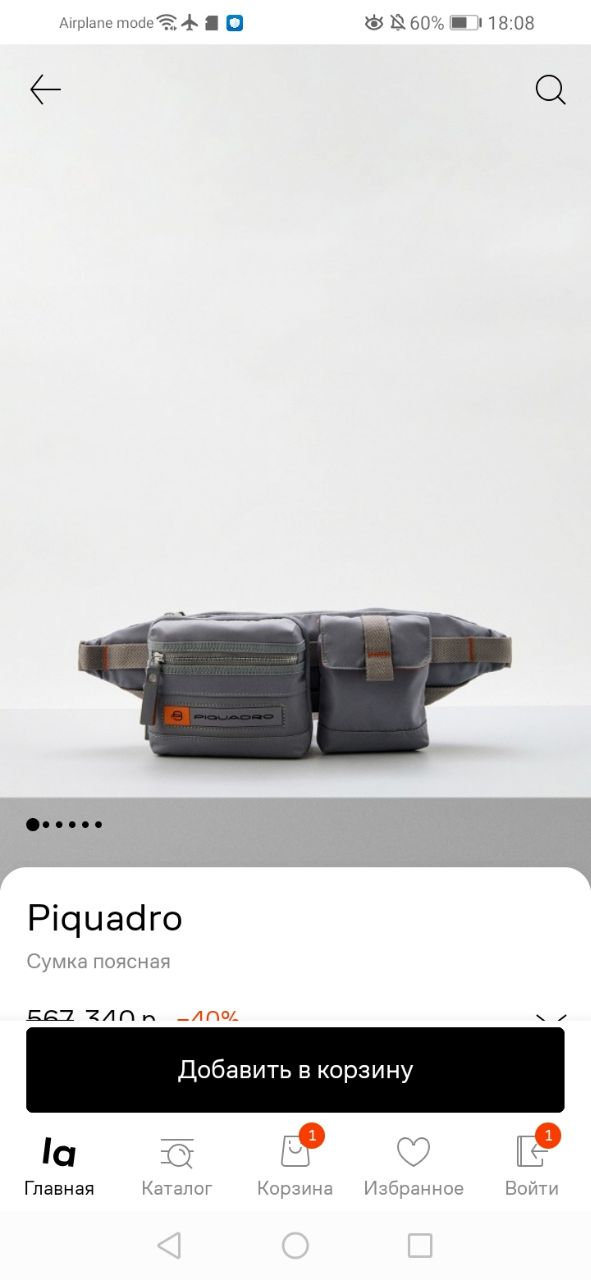
\includegraphics[width=.99\linewidth]
    {images/candidates/Lamoda/Item.jpg}
  \end{minipage}
  \begin{minipage}{0.16\textwidth}
    
\includegraphics[width=.99\linewidth]
    {images/candidates/DeFacto/Item.jpg}
  \end{minipage}
  \begin{minipage}{0.16\textwidth}
    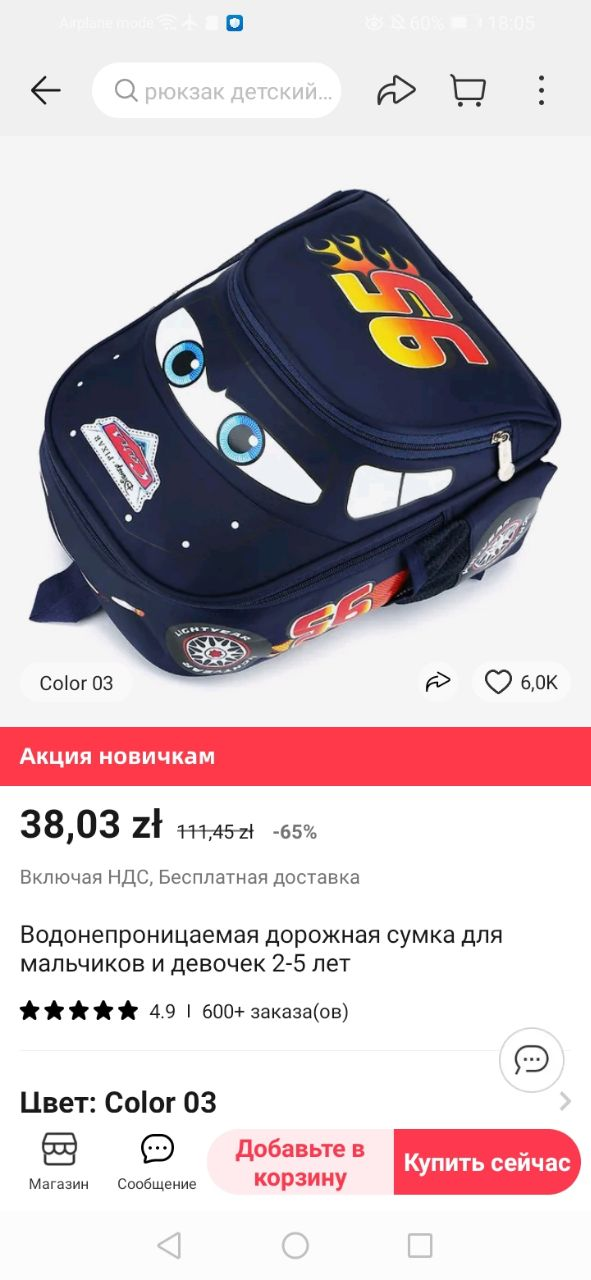
\includegraphics[width=.99\linewidth]
    {images/candidates/AliExpress/Item.jpg}
  \end{minipage}

  \caption{Аналоги экрана с товаром}\label{fig:analyzItem}
\end{figure}

\begin{figure}[!p]
  \centering

  \begin{minipage}{0.16\textwidth}
    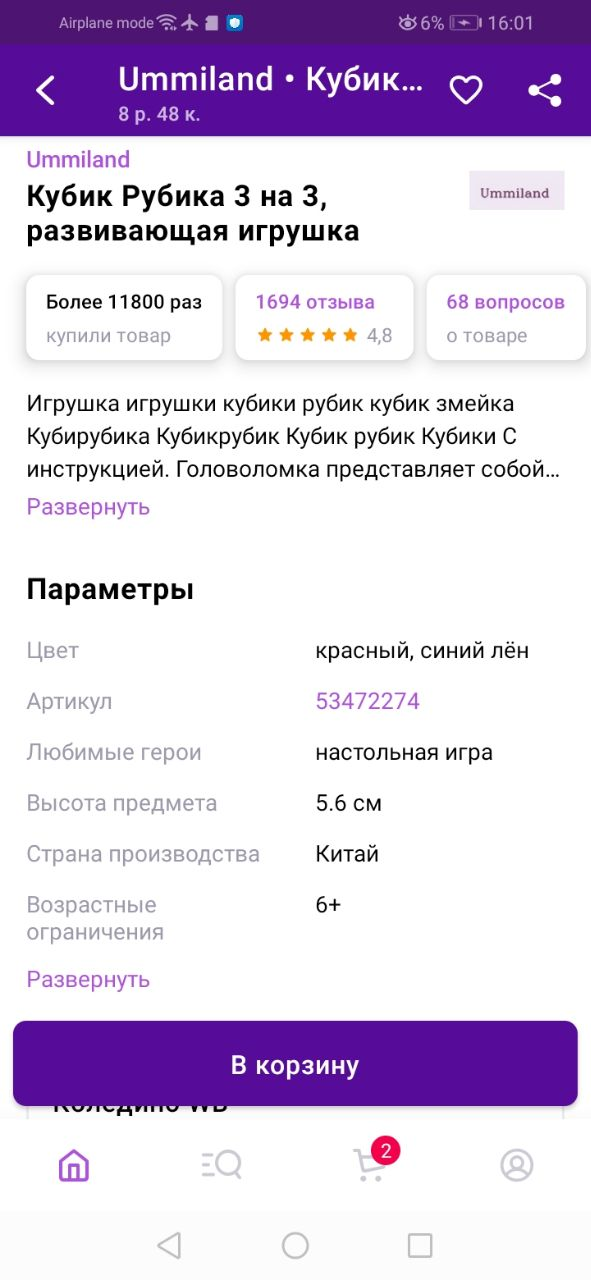
\includegraphics[width=.99\linewidth]
    {images/candidates/Wildberies/ItemCharacteristics.jpg}
  \end{minipage}
  % \begin{minipage}{0.16\textwidth}
  %   \includegraphics[width=.99\linewidth]
  %   {images/candidates/OZby/ItemCharacteristics.jpg}
  % \end{minipage}
  % \begin{minipage}{0.16\textwidth}
  %   \includegraphics[width=.99\linewidth]
  %   {images/candidates/LCWaikiki/ItemCharacteristics.jpg}
  % \end{minipage}
  \begin{minipage}{0.16\textwidth}
    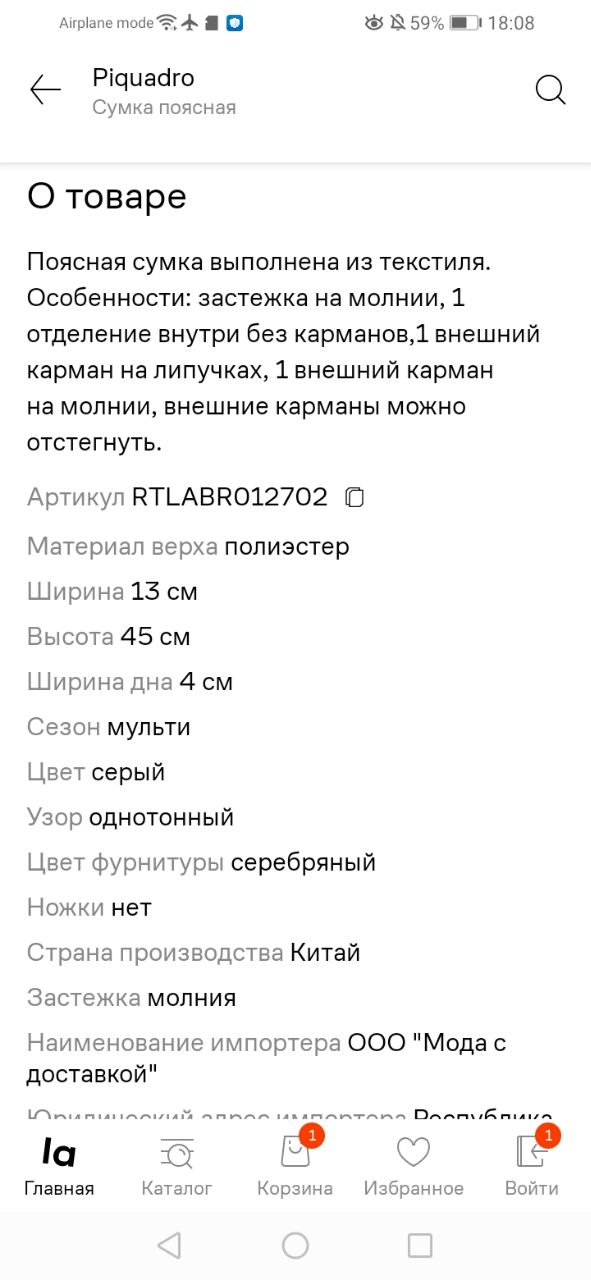
\includegraphics[width=.99\linewidth]
    {images/candidates/Lamoda/ItemCharacteristics.jpg}
  \end{minipage}
  \begin{minipage}{0.16\textwidth}
    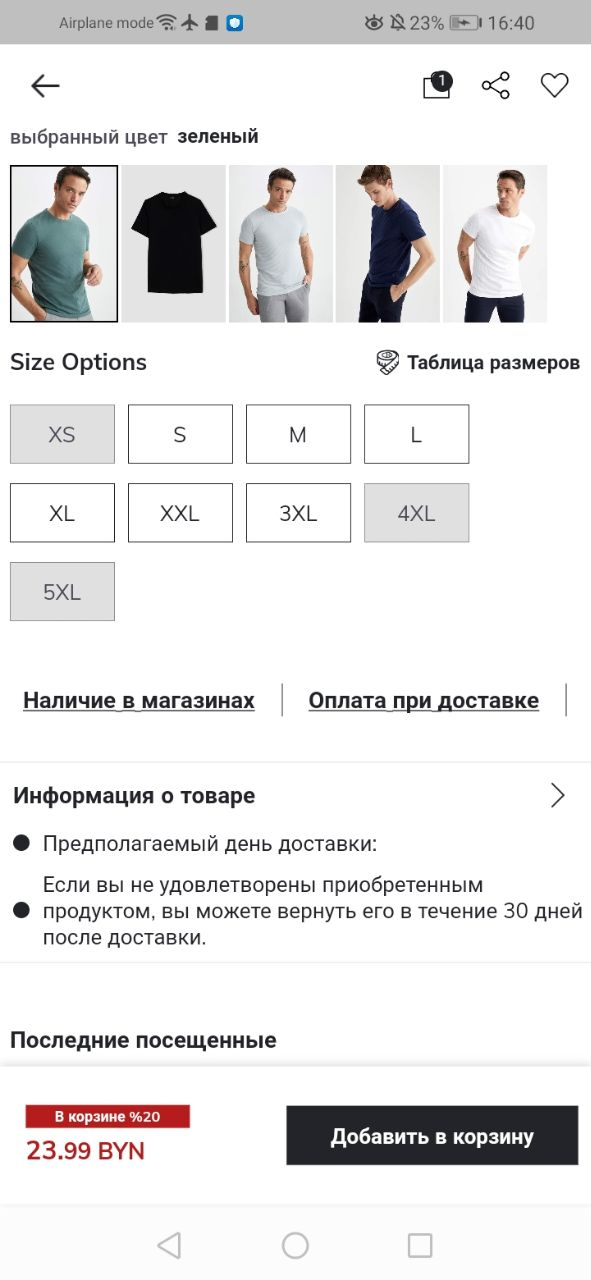
\includegraphics[width=.99\linewidth]
    {images/candidates/DeFacto/ItemCharacteristics.jpg}
  \end{minipage}
  \begin{minipage}{0.16\textwidth}
    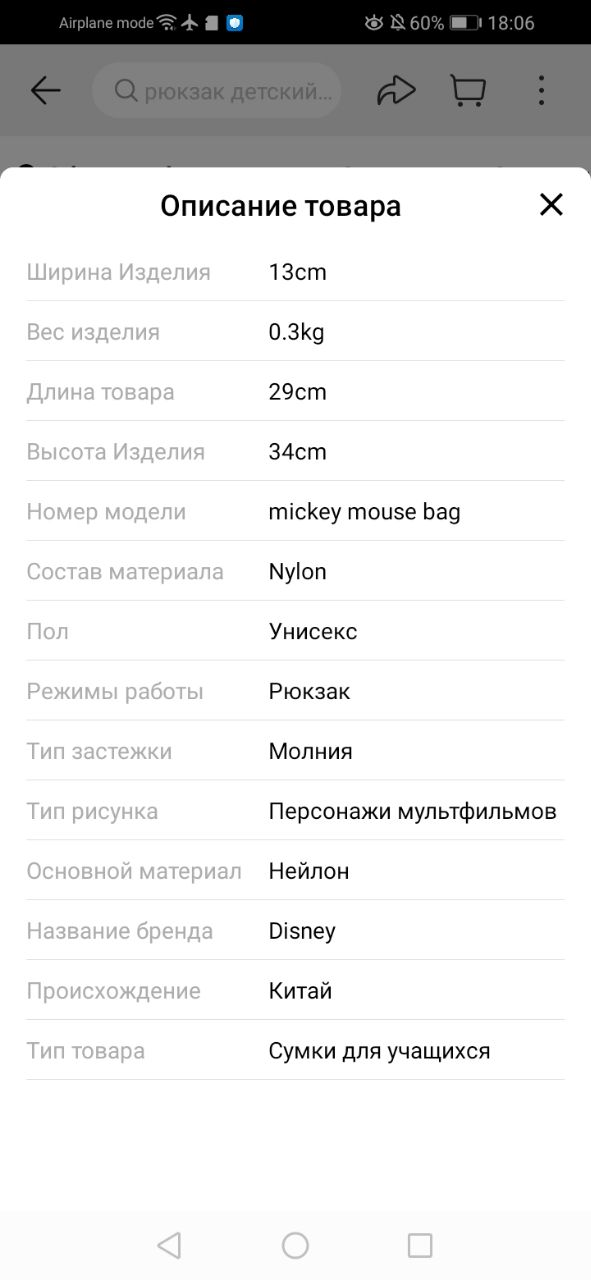
\includegraphics[width=.99\linewidth]
    {images/candidates/AliExpress/ItemCharacteristics.jpg}
  \end{minipage}

  \caption{Примеры описания характиристик номенклатуры}\label{fig:analyzItemCharacteristic}
\end{figure}

Экран с корзиной номенклатуры - это функциональность в мобильном приложении,
которая позволяет покупателю собирать товары, которые он хочет купить.
Покупатель может добавлять и удалять товары из корзины, изменять количество товаров,
просматривать общую стоимость и оформлять заказ.

Показ корзины без регистрации важен,
так как многие покупатели не желают тратить время на регистрацию в приложении,
прежде чем начать совершать покупки.
Показ корзины без регистрации также дает покупателям возможность быстро и легко просматривать товары,
которые они добавили в корзину, и оценивать общую стоимость заказа, прежде чем оформлять покупку.

Аналоги экрана с корзиной приведены на рисунке~\ref{fig:analyzBasket}.

Экран авторизации - это страница, на которой пользователь вводит свои данные для входа
в приложение или сайт.
Это может включать в себя поле для ввода электронной почты или логина, 
 также поле для ввода пароля.
Экран авторизации может также включать в себя функции восстановления пароля
или регистрации нового пользователя. 

Аналоги экрана авторизации приведены на рисунке~\ref{fig:analyzLogin}.

Экран с избранным в мобильном приложении представляет собой список товаров,
которые пользователь отметил для последующего просмотра или покупки.
Он предназначен для того, чтобы пользователь мог сохранить товары, которые ему интересны,
но которые он не хочет покупать сразу.

Избранные товары должны быть доступны только авторизованным пользователям,
так как это позволяет сохранять выбранные товары на протяжении нескольких сессий
и переносить их на другие устройства.
Также это предотвращает потерю списка избранного при случайном выходе из приложения
или при сбое в работе устройства.
В отличие от корзины, которая представляет собой список товаров, находящихся в процессе покупки,
избранные товары не требуют немедленной покупки,
а могут быть отложены на неопределенное время.

Когда пользователь не авторизован, нажатие на кнопку сердечко приводит к появлению экрана авторизации.
После того, как пользователь войдет в свой аккаунт,
он может вернуться на страницу товара и добавить его в избранное.
Если пользователь еще не зарегистрирован,
то после нажатия на кнопку сердечко ему будет предложено зарегистрироваться и создать аккаунт.

Аналоги экрана избранных приведены на рисунке~\ref{fig:analyzLike}.

\begin{figure}[!p]
  \centering

  \begin{minipage}{0.16\textwidth}
    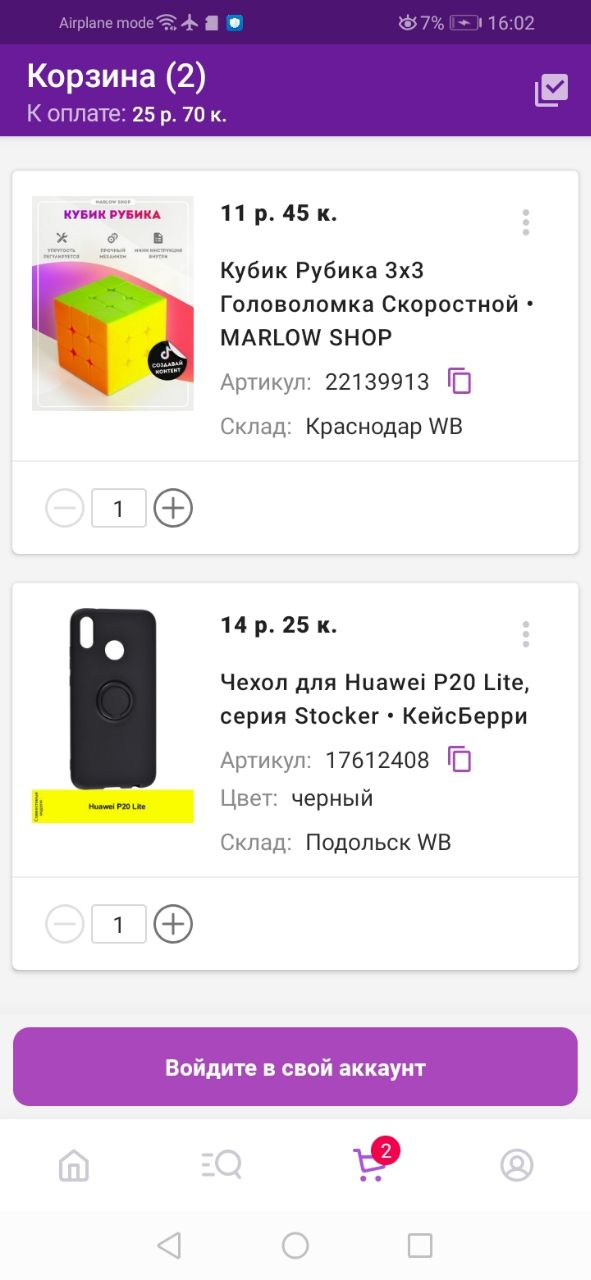
\includegraphics[width=.99\linewidth]
    {images/candidates/Wildberies/Basket.jpg}
  \end{minipage}
  % \begin{minipage}{0.16\textwidth}
  %   \includegraphics[width=.99\linewidth]
  %   {images/candidates/OZby/ItemCharacteristics.jpg}
  % \end{minipage}
  \begin{minipage}{0.16\textwidth}
    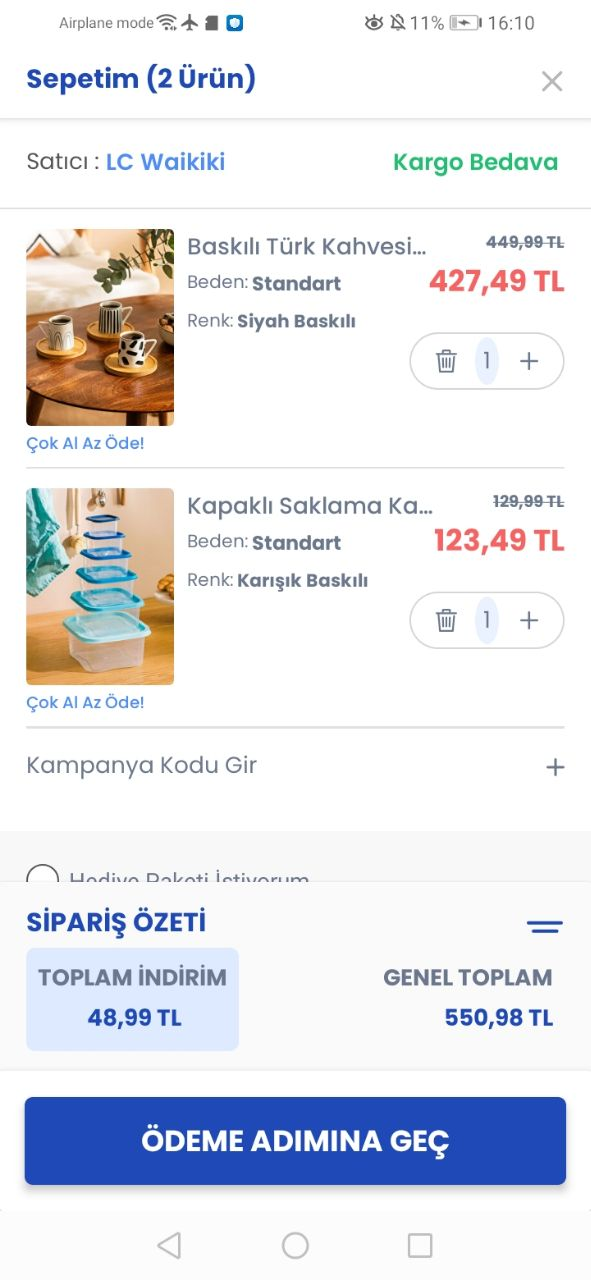
\includegraphics[width=.99\linewidth]
    {images/candidates/LCWaikiki/Basket.jpg}
  \end{minipage}
  \begin{minipage}{0.16\textwidth}
    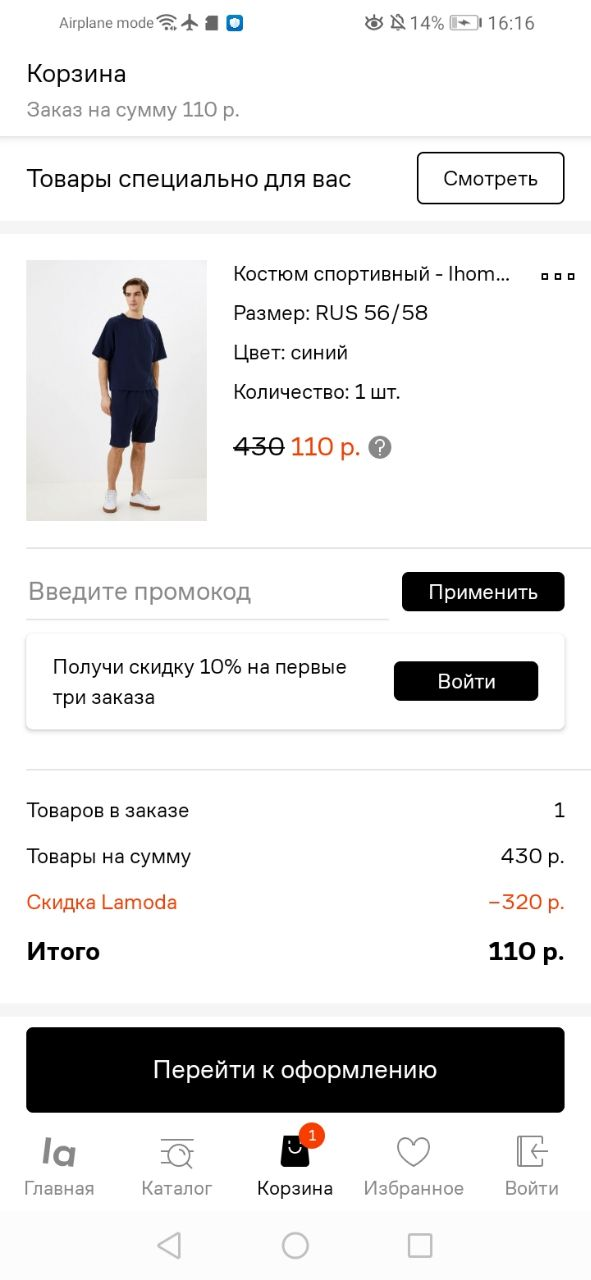
\includegraphics[width=.99\linewidth]
    {images/candidates/Lamoda/Basket.jpg}
  \end{minipage}
  \begin{minipage}{0.16\textwidth}
    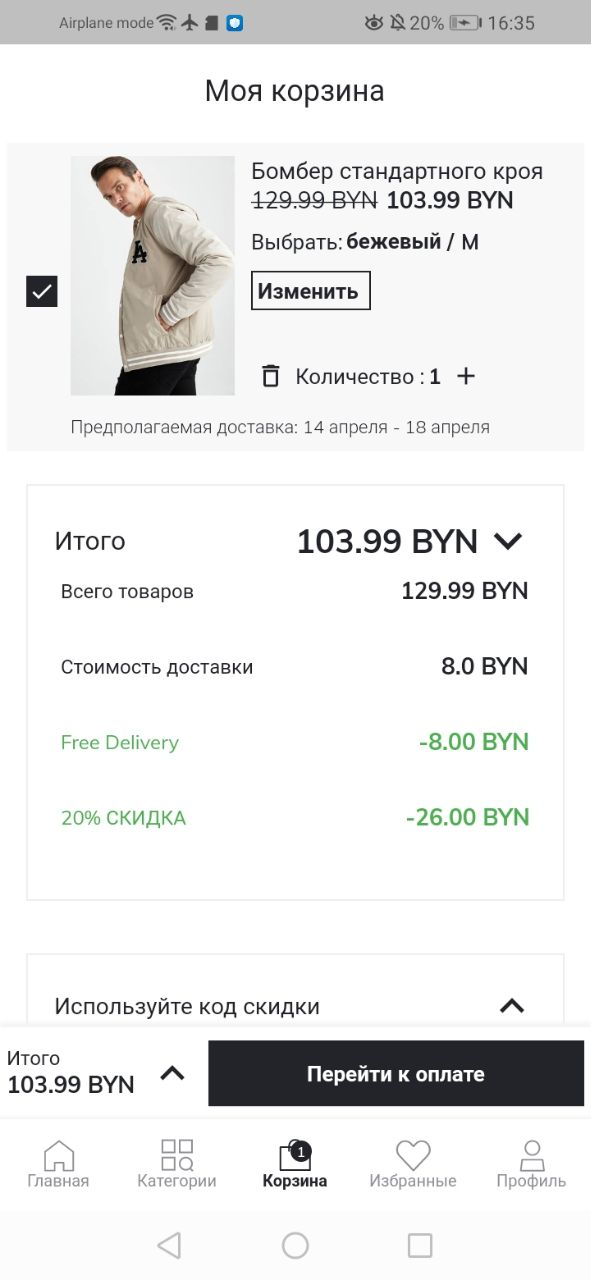
\includegraphics[width=.99\linewidth]
    {images/candidates/DeFacto/Basket.jpg}
  \end{minipage}
  \begin{minipage}{0.16\textwidth}
    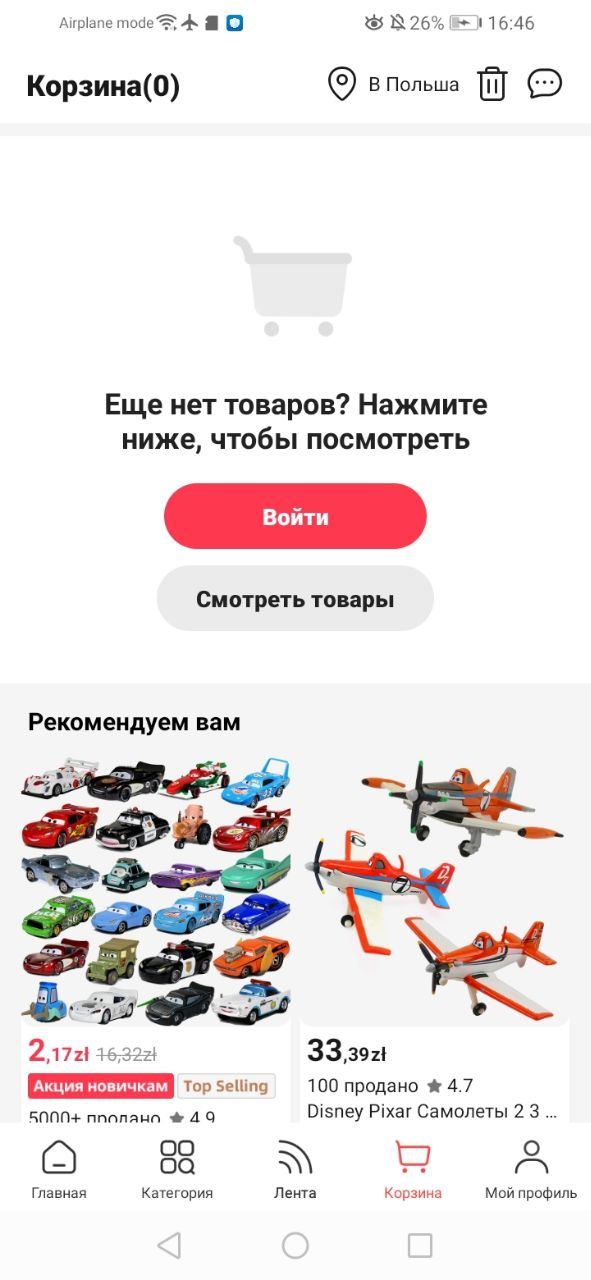
\includegraphics[width=.99\linewidth]
    {images/candidates/AliExpress/Basket.jpg}
  \end{minipage}

  \caption{Примеры оформления корзины с номенклатурой}\label{fig:analyzBasket}
\end{figure}

\begin{figure}[!p]
  \centering

  \begin{minipage}{0.16\textwidth}
    
\includegraphics[width=.99\linewidth]
    {images/candidates/Wildberies/Login.jpg}
  \end{minipage}
  \begin{minipage}{0.16\textwidth}
    
\includegraphics[width=.99\linewidth]
    {images/candidates/OZby/Login.jpg}
  \end{minipage}
  \begin{minipage}{0.16\textwidth}
    
\includegraphics[width=.99\linewidth]
    {images/candidates/LCWaikiki/Login.jpg}
  \end{minipage}
  \begin{minipage}{0.16\textwidth}
    
\includegraphics[width=.99\linewidth]
    {images/candidates/Lamoda/Login.jpg}
  \end{minipage}
  \begin{minipage}{0.16\textwidth}
    
\includegraphics[width=.99\linewidth]
    {images/candidates/DeFacto/Login.jpg}
  \end{minipage}
  % \begin{minipage}{0.16\textwidth}
  %   \includegraphics[width=.99\linewidth]
  %   {images/candidates/AliExpress/Login.jpg}
  % \end{minipage}

  \caption{Аналоги экрана входа}\label{fig:analyzLogin}
\end{figure}

\begin{figure}[!p]
  \centering

  % \begin{minipage}{0.16\textwidth}
  %   \includegraphics[width=.99\linewidth]
  %   {images/candidates/Wildberies/Like.jpg}
  % \end{minipage}
  % \begin{minipage}{0.16\textwidth}
  %   \includegraphics[width=.99\linewidth]
  %   {images/candidates/OZby/Like.jpg}
  % \end{minipage}
  \begin{minipage}{0.16\textwidth}
    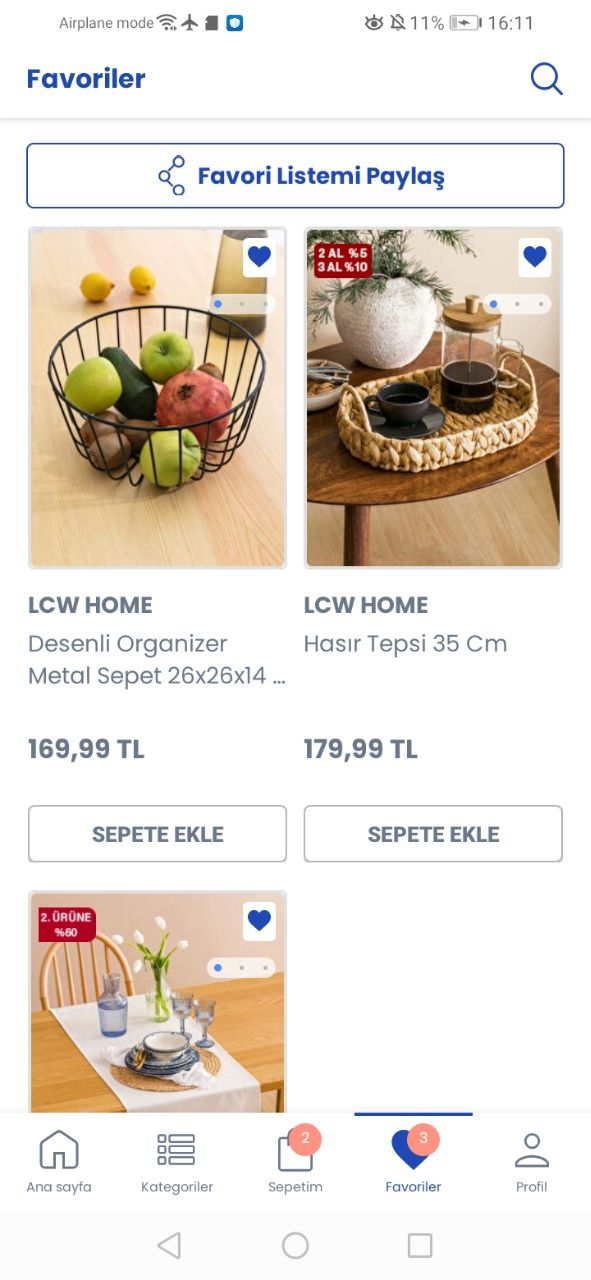
\includegraphics[width=.99\linewidth]
    {images/candidates/LCWaikiki/Like.jpg}
  \end{minipage}
  \begin{minipage}{0.16\textwidth}
    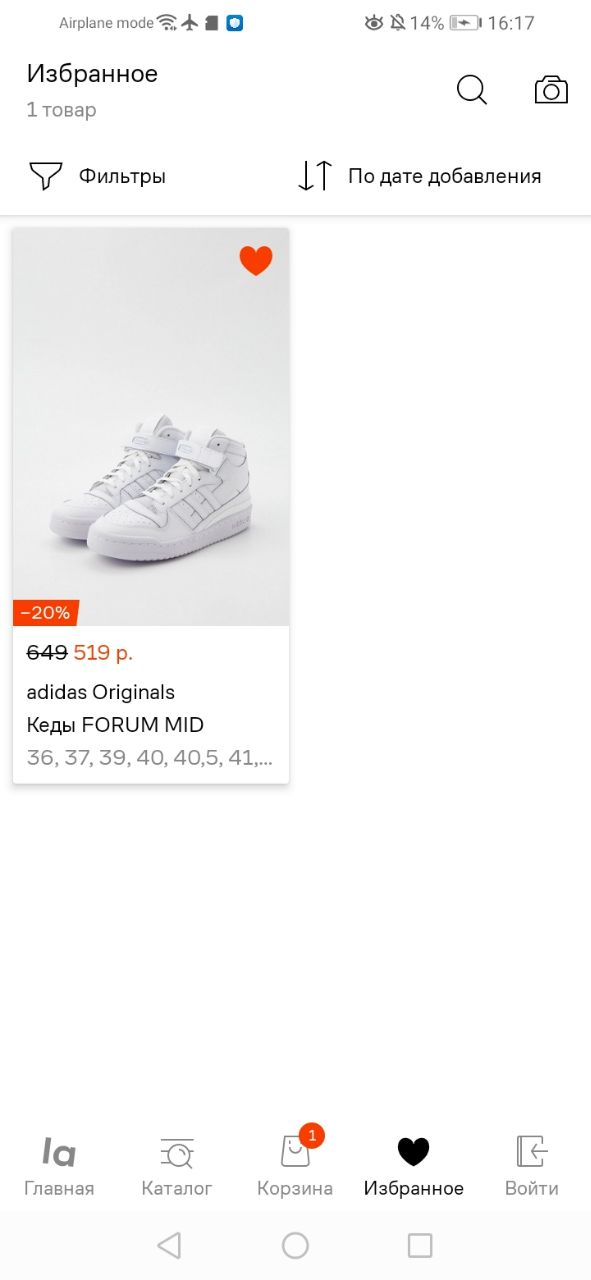
\includegraphics[width=.99\linewidth]
    {images/candidates/Lamoda/Like.jpg}
  \end{minipage}
  \begin{minipage}{0.16\textwidth}
    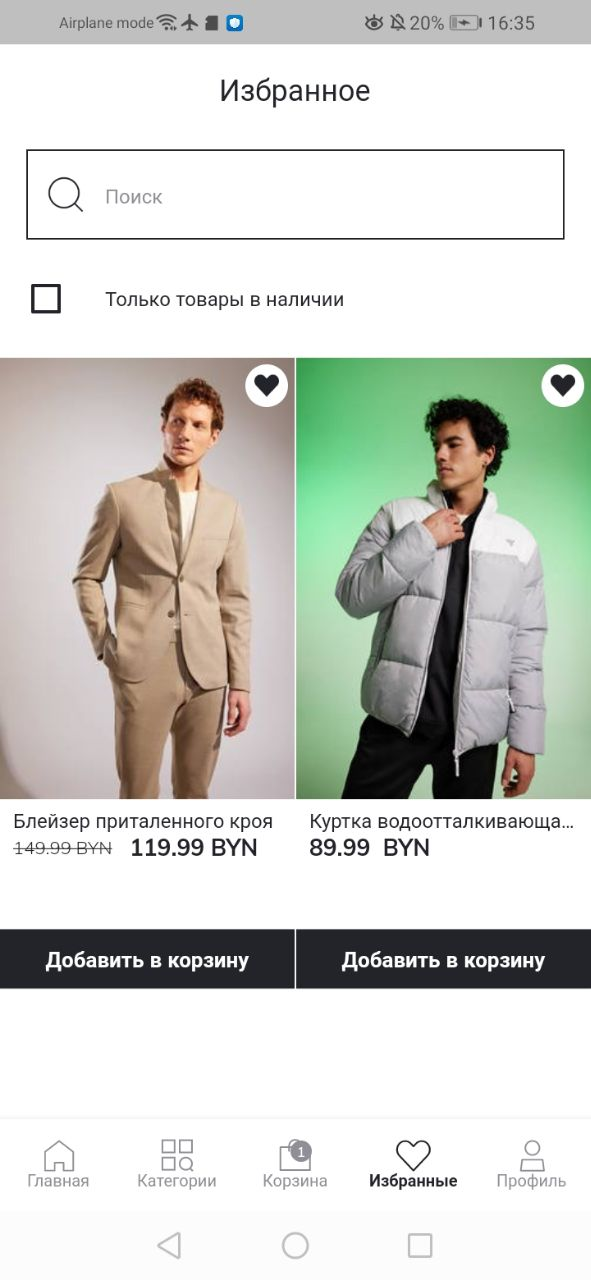
\includegraphics[width=.99\linewidth]
    {images/candidates/DeFacto/Like.jpg}
  \end{minipage}
  % \begin{minipage}{0.16\textwidth}
  %   \includegraphics[width=.99\linewidth]
  %   {images/candidates/AliExpress/Like.jpg}
  % \end{minipage}

  \caption{Примеры экрана избранных}\label{fig:analyzLike}
\end{figure}

\subsection{Обзор используемых технологий}

Нельзя точно уточнить, какие технологии использовались для написания мобильных приложений
WildBerries, OZ.by, LC Waikiki, Lamoda, Defacto,
потому что эта информация не является открытой и не раскрывается компаниями-разработчиками.
Компании могут использовать различные языки программирования и технологии в зависимости от своих потребностей,
бизнес-задач и команд разработки. Однако, стало изветно, что мобильное приложение AliExpress
написано на языке программирования Java когда оно сломалось \cite{AliExpressLang} \cite{AliExpressLangForum}.

Выбор технологий для разработки мобильных приложений зависит от многих факторов,
таких как требования к производительности, функциональные возможности, доступность ресурсов и т.д.
Поэтому разработчикам приходится выбирать технологии, которые лучше всего соответствуют их потребностям.
Однако в целом, для разработки мобильных приложений используются различные языки программирования и фреймворки,
такие как Java, Kotlin, Swift, React Native, Xamarin и др.

\subsection{Выбор средств реализации}

React Native \cite{ReactNativeCliGuide} был выбран из-за его возможностей создания кроссплатформенных мобильных приложений для iOS и Android,
используя язык программирования JavaScript (в данном дипломном проекте TypeScript) и React-стиль программирования.
Это позволяет существенно сократить время и затраты на разработку, так как код может быть использован на нескольких платформах.
Кроме того, React Native обеспечивает высокую производительность и хорошую оптимизацию для мобильных устройств.

MySQL \cite{MySqlInNestJs} был выбран в качестве базы данных, так как это надежная и широко используемая реляционная СУБД с открытым исходным кодом.
MySQL имеет высокую производительность, масштабируемость и поддерживает все необходимые функции для хранения, организации и извлечения данных.

Swagger \cite{SwaggerInNestJs} был выбран для создания документации API.
Это популярный инструмент для описания и документирования RESTful API.
Swagger обеспечивает удобное взаимодействие между разработчиками,
а также может использоваться для автоматической генерации клиентского кода на различных языках программирования.

NestJS \cite{NestJsGuide} был выбран как фреймворк для создания серверной части приложения.
Он построен на основе TypeScript и использует паттерн MVC (Model-View-Controller) для создания быстрых и масштабируемых веб-приложений.
Nest предоставляет множество инструментов для удобной работы с базами данных, а также обладает высокой производительностью и легким масштабированием.

TypeScript \cite{TypeScriptGuide} был выбран как язык программирования для всего комплекса програм,
как и серверной части, мобильного приложения и сайта с панелью администратора и менеджера.
TypeScript является надстройкой над JavaScript и обеспечивает статическую типизацию, что улучшает безопасность кода и позволяет облегчить его понимание и сопровождение.
TypeScript также обладает высокой читабельностью кода, что упрощает сопровождение и добавление новых функций в приложение.

TypeORM \cite{TypeORM} \cite{TypeOrmQueryRunner} был выбран в качестве ORM (Object-Relational Map-ping) для работы с базой данных в NestJS.
TypeORM позволяет работать с базами данных разных типов, включая реляционные и NoSQL СУБД, используя объектно-ориентированный подход к работе с данными.
Это позволяет более удобно и эффективно работать с базой данных, а также улучшить производительность и масштабируемость приложения.
TypeORM также предоставляет множество инструментов для управления миграциями базы данных и обновлением схемы данных, что делает процесс разработки и сопровождения приложения более гибким и удобным.

Дополнительно, следует отметить, что TypeORM позволяет создавать миграции базы данных,
что является очень полезной функцией при разработке и сопровождении приложения.

Миграции позволяют автоматически изменять структуру базы данных
без необходимости ручного вмешательства в саму базу данных.

Таким образом, можно легко добавлять новые таблицы,
изменять существующие или удалять их, не беспокоясь о том,
что это может повлиять на работу приложения или привести к ошибкам в работе.

В итоге, React Native, MySQL, Swagger, NestJS, TypeScript и TypeORM были выбраны для создания мобильного приложения под Android из-за их возможностей и надежности,
а также для обеспечения удобной разработки, документирования и масштабирования.

\newpage
